% !TEX root = ../intro-stellar-physics.tex

We now have almost all of the physics necessary to describe the structure of a star. We only need two additional items: we must consider whether the fluid can slowly circulate and thereby trasnport heat, and we must discuss how the equation of state deviates from that of a classical ideal gas at high densities and at high temperatures. The changes in the equation of state at high densities are important for low-mass stars and set the minimum stellar mass; the changes at high temperatures are important for high-mass stars and set the maximum stellar mass.

\section{Convection}\label{s.convection}

We've established that in the interior of the star a temperature gradient,
\[
	\DD{T}{r} = -\frac{3\rho\kappa_{R}}{4acT^3}\frac{L(r)}{4\pi r^2},
\]
arises to transport heat outward (cf.\ eq.~[\ref{e.gradient-temperature}]).
This gradient becomes steeper as we increases either the flux $L/4\pi r^{2}$ or the mean opacity $\kappa_{\mathrm{R}}$. There is a limit, however, to the magnitude of $|\dif T/\dif r|$: if the gradient is too steep, the warm fluid becomes buoyant relative to the cooler fluid above it and begins to rise. You are familiar with this phenomenon: picture a hot summer day. As the ground absorbs sunlight, it warms the air just above the ground. The warm air rises and forms updrafts. You have perhaps seen hawks circling as they are carried aloft by these updrafts. This circulation of fluid induced by a temperature gradient is known as \newterm{convection}. 

You can do a home demonstration of convection.\marginnote{As a bonus, you can drink the results of this demonstration.} Brew tea, and pour the hot tea into a saucepan that is on an unlit burner. Use a straw to inject a layer of cold milk under the hot tea in the saucepan. The temperature difference between the tea and milk inhibits premature mixing. Light the burner, and watch for the development of convection---you will know it when you see it (Fig.~\ref{f.tea}).

\begin{figure}[htbp]
\forceversofloat
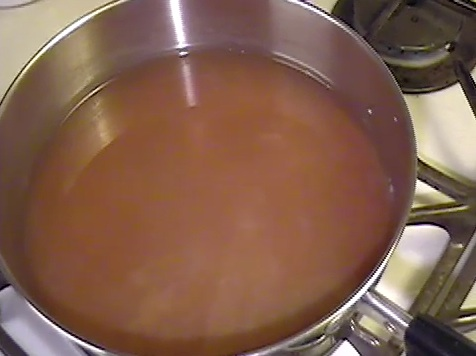
\includegraphics[width=0.5\linewidth]{convection-1}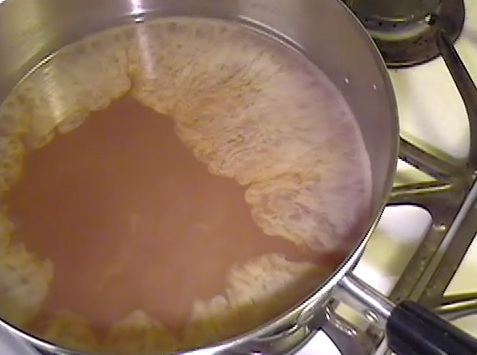
\includegraphics[width=0.5\linewidth]{convection-2}
\caption[Onset of convection]{Onset of convection in a tea-milk mixture.\label{f.tea}}
\end{figure}

Convection can also occur in stars, in regions of high flux and/or high opacity. During convection, the fluid velocities in question are typically quite subsonic, so hydrostatic equilibrium abides. But the fluid motions do make an enormous difference to heat transport! Warm fluid is carried upward and cool fluid sinks. The net result is that heat is transported upward much faster than it would have been if only diffusion had been operating. This upward transport of heat modifies the temperature gradient. In this chapter, we shall derive the condition for the onset of convection, and the value of the temperature gradient in the presence of subsonic, efficient convection.

\subsection{The onset of convection}\label{s.convection-onset}

To understand when convection starts, it helps to recall why a parcel of warm air rises. Recall Archimedes' law:
\begin{quote}\itshape
The buoyant force on an object, either wholly or partially immersed in a fluid under a constant gravitational acceleration, equals the weight of the fluid it displaces.
\end{quote}
What does this mean? When floating (buoyant force equals weight), a boat of mass $m$ displaces (pushes aside) a volume $v$ of water of density $\rho_{\mathrm{w}}$. The weight of this displaced water, $\rho_{\mathrm{w}}v g$, must equal the weight of the boat $mg$, so that $v = m/\rho_{\mathrm{w}}$.

\begin{exercisebox}[A boat with a weight]
Suppose we have a toy boat carrying a weight and floating in a tank as shown in the top panel of Fig.~\ref{f.archimedes}. The depth of the water in the tank is $d$. The weight is then removed from the boat and allowed to sink to the bottom of the tank (bottom panel, Fig.~\ref{f.archimedes}). Does the depth of water in the tank increase, decrease, or stay the same? Explain your reasoning.
\end{exercisebox}
\begin{marginfigure}[-6\baselineskip]
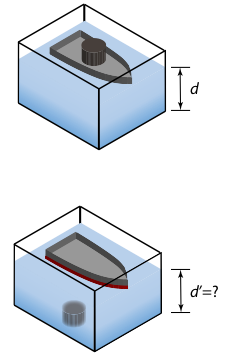
\includegraphics[width=\linewidth]{archimedes}
\caption[A boat with a weight]{\label{f.archimedes} A boat with a weight in a tank.}
\end{marginfigure}

We can use Archimedes' law---which is just an application of hydrostatic equilibrium---to determine whether a fluid in planar geometry and hydrostatic equilibrium,
\begin{equation}
\frac{\dif P}{\dif r} = -\rho g,
\end{equation}
and with a temperature gradient is unstable to convection. We start with a fluid at rest in hydrostatic equilibrium in spherical symmetry, so $P$, $\rho$, and $T$ depend on radial position $r$.
Imagine moving a blob of fluid upwards from $r$ to $r+h$. We raise the blob slowly enough that it is in hydrostatic equilibrium with its new surroundings,\sidenote{We'll use the subscript $b$ to denote properties of the blob; quantities without a subscript refer to the background fluid.} $P_{b}(r+h) = P(r+h)$. We do move the blob quickly enough, however, that it doesn't exchange heat with its surroundings and therefore doesn't remain in \emph{thermal} equilibrium with its new environment. 

As a result of this lack of heat exchange, the upward motion of the blob is \newterm{adiabatic}.  \marginnote{Pressure equilibrium in the blob is established over the time a sound wave takes to cross the blob. Thus, moving the blob slowly enough to maintain pressure equilibrium means that the motion is quite subsonic. Moving the blob quickly enough to prevent heat transport means (cf.\ exercise~\ref{ex.random-walk-diffusion}) that the blob is much larger than a mean free path so the time for photons to random walk across the blob is longer than time taken to raise the blob.}
To understand what this means, recall the first law of thermodynamics, which relates the change in internal energy $\dif U$ and in volume $\dif V$ to the heat transferred $\dif Q = T\,\dif S$:
\begin{equation}\label{e.first-law-thermo}
	\dif Q = T\,\dif S = \dif U + P\,\dif V,
\end{equation}
where $P$ is the pressure, $T$ the temperature, and $S$ the entropy. During an adiabatic process, $\dif Q = T\,\dif S = 0$. The entropy of the blob is therefore constant, 
$S_{b}(r+h) = S_{b}(r) = S(r)$, and is therefore not equal, in general, to the entropy of the surrounding gas at $r+h$: $S_{b}(r+h)  \neq S(r+h)$.

As in our discussion of the equation of state (cf.\ eq.~[\ref{e.ideal-gas-eos}]), it isn't really convenient to write things in terms of volume. To put eq.~(\ref{e.first-law-thermo}) into a more convenient form, divide both sides by the mass of the blob $m_{b}=\rho V$:
\begin{eqnarray}
	\dif\left(\frac{Q}{m_{b}}\right) = T\,\dif\left(\frac{S}{m_{b}}\right) &=&
		\dif\left(\frac{U}{m_{b}}\right) + P\,\dif\left(\frac{V}{m_{b}}\right)\nonumber\\
	T\,\dif s &=& \dif u + P\,\dif\left(\frac{1}{\rho}\right)\nonumber\\
	T\,\dif s &=& \dif u - \frac{P}{\rho^{2}}\dif\rho \label{e.specific-first-law-thermo}
\end{eqnarray}
Here we denote the \emph{entropy per mass} and the \emph{energy per mass} by $s$ and $u$ respectively; and we identify the volume per mass with $1/\rho$, where $\rho$ is the mass density. Equation~(\ref{e.specific-first-law-thermo}) is the first law of thermodynamics as written for fluid dynamics.

\begin{marginfigure}
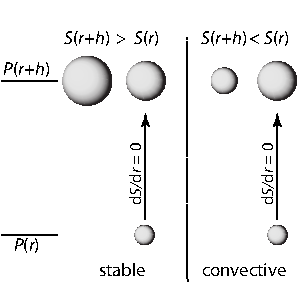
\includegraphics[width=\textwidth]{convective}
\caption[Illustration of criteria for convective instability]{\label{f.convective-schematic}Illustration of criteria for convective instability.  On the left, raising a blob a distance $h$ adiabatically and in pressure balance with its surrounding results in a higher density $V_{b} < V$, or $\rho_{b} > \rho$.  This is stable: the blob will sink back.  On the right, the blob is less dense and hence buoyant: it will continue to rise.}
\end{marginfigure}
The blob expands as it moves upward from $r$ to $r+h$:
\[
	\rho_{b}(r+h) = \rho[P_{b}(r+h),s_{b}(r+h)] = \rho[P(r+h),s(r)].
\]
Here we've written the density as a function of pressure and entropy, $\rho(P,s)$. Now we can apply Archimedes' law: if the density of the blob at $r+h$ is greater than that of the surrounding fluid, then the buoyant force will be less than the weight of the blob; as a consequence, the blob will sink back to its original location. The fluid is thus stable. In contrast, if the density of the blob at $r+h$ is less than that of the surrounding fluid, then the buoyant force is greater than the weight of the blob; as a result, the blob will continue to rise. In this case, the fluid is unstable: a small perturbation leads to the acceleration of the blob upwards. Figure~\ref{f.convective-schematic} has a schematic of this criterion.

Thus, for the fluid to be stable, we require that the density of the displaced blob be greater than that of the surrounding fluid:
\begin{eqnarray}
\rho_{b}(r+h) &>& \rho(r+h) \nonumber\\
\rho[P(r+h),s(r)] &>& \rho[P(r+h),s(r+h)].
\label{e.archimedes}
\end{eqnarray}
If condition (\ref{e.archimedes}) is satisfied, then the blob will be restored to its original location after a perturbation, and the system is stable. If condition (\ref{e.archimedes}) is not satisfied, then the blob will continue to rise following a perturbation, and the system is unstable.

We take $h$ to be an infinitesimal displacement, so we can expand the right-hand side of eq.~(\ref{e.archimedes}) about $\rho[P(r+h),s(r)]$:
\[
	\rho[P(r+h),s(r+h)] \approx \rho[P(r+h),s(r)] + \tderiv{\rho}{s}{P}\DD{s}{r}\;h.
\]
Here the notation $(\partial \rho/\partial s)_{P}$ means taking the derivative of $\rho$ with respect to $s$ while holding $P$ fixed. After canceling common factors, equation~(\ref{e.archimedes}) therefore reduces to
\begin{equation}\label{e.convective-stability}
 \tderiv{\rho}{s}{P}\frac{\dif s}{\dif r} \;h < 0 .
\end{equation}
We can put eq.~(\ref{e.convective-stability}) into a more useful form by changing variables from entropy $\rho$ to temperature $T$ via
\[
\tderiv{\rho}{T}{P} = \tderiv{\rho}{s}{P}\tderiv{s}{T}{P} = \tderiv{\rho}{s}{P}\frac{C_{P}}{T},
\]
where we introduce the specific heat at constant pressure, $C_{P}\equiv T(\dif s/\dif T)_{P}$.
Inserting this expression into eq.~(\ref{e.convective-stability}) and dropping $h$ (since it is positive by construction) gives
\[
 \frac{T}{C_{P}}\tderiv{\rho}{T}{P}\frac{\dif s}{\dif r} < 0,
\]
Now, $(\partial \rho/\partial T)_{P}$ is negative (gas expands on being heated), while $C_{P}$ is positive; hence eq.~(\ref{e.convective-stability}) will be satisfied wherever
\begin{equation}\label{e.entropy-condition}
\frac{\dif s}{\dif r} > 0.
\end{equation}
\begin{quote}\itshape
In a convectively stable star, the entropy must increase with radius.
\end{quote}
If this condition is not satisfied---if $\dif s/\dif r < 0$---then convection ensues: high-entropy material is buoyant and rises upward, while lower-entropy material sinks inward. Eventually this circulation mixes the rising high-entropy fluid with the sinking low-entropy fluid and drives the entropy gradient toward the marginally stable configuration $\dif s/\dif r = 0$.

\subsection{The adiabatic thermal gradient}\label{s.adiabatic-gradient}

Although succinct, the condition (\ref{e.entropy-condition}) for convective stability is not directly useful since our equations of stellar structure do not directly involve the entropy. We'd instead like to express the criterion for the onset of convection in terms of pressure and temperature, since those quantities appear in our stellar structure equations. 

\begin{sidebar}[Along an adiabat]
\label{sb.adiabatic-changes}
To describe adiabatic processes, let's start from the first law expressed in terms of mass-specific quantities (eq.~[\ref{e.specific-first-law-thermo}]):
\[
	\dif q = T\,\dif s = \dif u -\frac{P}{\rho^{2}}\,\dif \rho.
\]
We write the energy $u$ as a function of temperature $T$ and density $\rho$, $u = u(\rho,T)$, and take the differential,
\[ \dif u = \tderiv{u}{T}{\rho}\dif T + \tderiv{u}{\rho}{T}\dif \rho. \]
We insert this expression for $\dif u$ into eq.~(\ref{e.specific-first-law-thermo}) and find
\[ \dif q = T\dif s = \tderiv{u}{T}{\rho}\dif T + \left[\tderiv{u}{\rho}{T} - \frac{P}{\rho^{2}}\right]\dif \rho. \]
Hence the heat needed to raise the temperature of one kilogram of fluid while holding density fixed is
\begin{equation}\label{e.CV}
C_{\rho} \equiv T\,\tderiv{s}{T}{\rho} = \tderiv{u}{T}{\rho}.
\end{equation}
For an ideal gas $C_{\rho}$ is a constant and the internal energy $u = u(T)$ is independent of density. In what follows, we'll specialize to the case of an ideal gas.

To express the first law in terms of $T$ and $P$, rather than $T$ and $\rho$, write eq.~(\ref{e.specific-first-law-thermo}) as
\begin{equation}\label{e.first-law-specific-heat}
T\,\dif s = C_{\rho}\dif T - \frac{P}{\rho}\frac{\dif\rho}{\rho} .
\end{equation}
Then take the logarithm of the ideal gas equation of state, $\ln (P) = \ln(\rho) + \ln (T) + \ln (\kB/\mu\mb)$, and differentiate to find
\[ \frac{\dif P}{P} = \frac{\dif\rho}{\rho} + \frac{\dif T}{T}. \]
Use this to eliminate $\dif\ln\rho$ in eq.~(\ref{e.first-law-specific-heat})
to obtain an expression for the heat transferred as a function of temperature and pressure,
\begin{equation}\label{e.first-law-pressure-temperature}
T\,\dif s = \left[C_{\rho} + \frac{P}{\rho T}\right]\dif T - \frac{1}{\rho}\dif P
	 = \left[C_{\rho} + \frac{\kB}{\mu\mb}\right]\dif T - \frac{1}{\rho}\dif P.
\end{equation}
The heat needed to raise the temperature of a mass of fluid while holding pressure fixed is therefore
\begin{equation}\label{e.CP}
C_{P}\equiv T\,\tderiv{s}{T}{P} = C_{\rho} + \frac{\kB}{\mu\mb}.
\end{equation}
For a plasma of ions and electrons, the specific heats are
\begin{eqnarray}
C_\rho &=& \frac{3}{2}\frac{\kB}{\mu\mb}  \label{e.specific-heat-density},\\
C_P    &=& \frac{5}{2}\frac{\kB}{\mu\mb}; \label{e.specific-heat-pressure}
\end{eqnarray}
the ratio of these specific heats is
\begin{equation}\label{e.gamma}
    \gamma = \frac{C_P}{C_\rho} = \frac{5/2}{3/2} = \frac{5}{3}.
\end{equation}
This value of $\gamma$ is for an ideal, monatomic gas and does not hold universally.
\end{sidebar}

\newthought{During adiabatic motion, there is no heat exchange:} hence, the entropy is constant and eq.~(\ref{e.first-law-pressure-temperature}) relates temperature and pressure:
\begin{equation}\label{e.differential-entropy}
    T\dif s = \dif q = 0 = C_{P}\dif T - \frac{1}{\rho} \dif P.
\end{equation}
Rearranging terms and using the ideal gas equation of state to eliminate $1/\rho$, we obtain
\begin{eqnarray}
     C_{P}\dif T &=& \frac{\kB}{\mu\mb}\frac{T}{P}\dif P; \nonumber\\
     \frac{\dif T}{T} &=& \frac{C_{P}-C_{\rho}}{C_{P}} \frac{\dif P}{P}\nonumber\\
	&=& \frac{\gamma-1}{\gamma}\frac{\dif P}{P}.
\label{e.differential-adiabat}
\end{eqnarray}
Here we've used the ratio of specific heats $\gamma$, eq.~(\ref{e.gamma}), and the equation of $C_{P}$, eq.~(\ref{e.CP}) for an ideal gas.
Integrating eq.~(\ref{e.differential-adiabat}) gives us $T(P)$ along an adiabat\sidenote{We used a similar relation in determining the sound speed (Box~\ref{b.sound-speed}).}:
\begin{equation}\label{e.adiabat}
 T = T_{0}\left(\frac{P}{P_{0}}\right)^{(\gamma-1)/\gamma}.
\end{equation}
Here $T_{0}$ and $P_{0}$ are the temperature and pressure at the beginning of the adiabatic process. 

\begin{exercisebox}[Adiabatic relations]
Use equation~(\ref{e.adiabat}) and the equation of state of an ideal gas to derive a relation between temperature and density, as well as a relation between density and pressure, during an adiabatic process.
\end{exercisebox}

In a convectively stable star, $\dif s/\dif r > 0$ (eq,~\ref{e.entropy-condition}]), and so 
\begin{equation}\label{e.convectively-stable}
	 C_{P} \DD{T}{r} = \frac{1}{\rho}\DD{P}{r} + T\DD{s}{r} > \frac{1}{\rho}\DD{P}{r}.
\end{equation}
Now, $\dif P/\dif r = -\rho g$ because the fluid is in hydrostatic equilibrium; and this is true even if convection is occurring, so long as the convective motions are quite subsonic.  Since the pressure $P$ decreases monotonically with radius, we can use the equation of hydrostatic balance to write $\dif T/\dif r = (\dif T/\dif P)(\dif P/\dif r)$.
Inserting this into equation~(\ref{e.convectively-stable}), changing the direction of the inequality since $\dif P/\dif r < 0$, and rearranging slightly gives
\begin{eqnarray}
\DD{T}{P} &<& \frac{1}{\rho C_{P}} \nonumber\\
\frac{P}{T}\DD{T}{P} &<& \frac{P}{C_{P}\rho T} = 
\frac{\gamma - 1}{\gamma} = \frac{P}{T}\tderiv{T}{P}{s} .\label{e.stability-dTdP}
\end{eqnarray}
Although we derived eq.~(\ref{e.stability-dTdP}) for the case of an ideal gas, it is in general true. The left-hand side is the relation between temperature and pressure in the star, as set by radiative conduction; the right-hand side is the relation between temperature and pressure along an adiabat.  The condition for stability, eq.~(\ref{e.stability-dTdP}), can be more succinctly written as
\begin{equation}\label{e.stability-del}
\nablarad \equiv \DD{\ln T}{\ln P} < \tderiv{\ln T}{\ln P}{s} \equiv \nablaad.
\end{equation}
for the fluid to be stable against convection.

\begin{exercisebox}[Onset of convection]
The figure shows some hypothetical runs of temperature with respect to pressure in a gas in hydrostatic equilibrium.  Indicate which of these situations is convectively unstable, and explain why. Draw on that plot the pressure-temperature relation that would ensue once convection sets in.

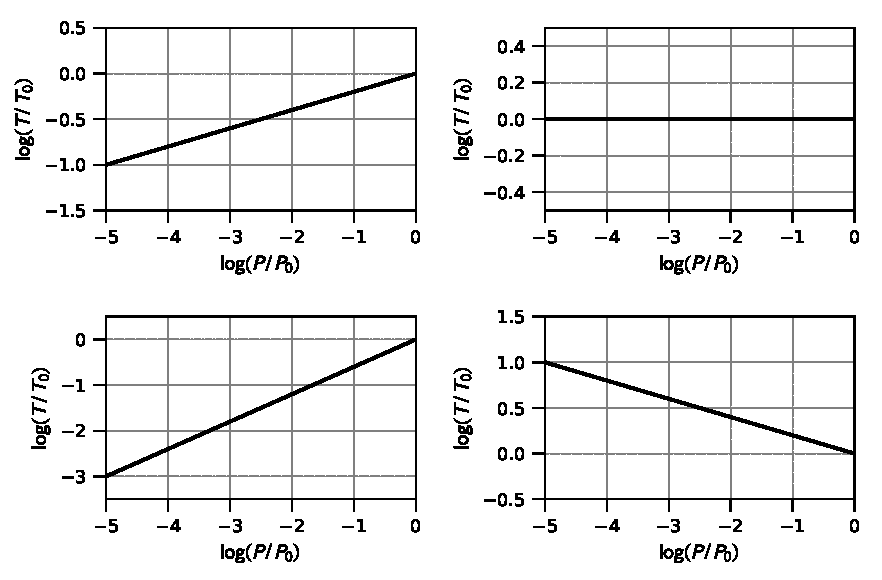
\includegraphics[width=\linewidth]{convection-worksheet-1}
\end{exercisebox}

When convection is absent, the temperature gradient in the star is (eq.~[\ref{e.gradient-temperature}])
\[
    \DD{T}{r} = -\frac{3\rho\kappa}{4acT^3}\frac{L(r)}{4\pi r^2}.
\]
Here $\kappa$ is the opacity and $L(r)$ is the luminosity at radius $r$: $L/4\pi r^2$ is the flux. If this thermal gradient, $|\dif T/\dif r|$, becomes too steep, however, then---just as in the pot of tea and milk on the stove, Fig.~\ref{f.tea}---the fluid becomes unstable: warm fluid begins to rise while cold fluid sinks. Over a wide range of stellar conditions this mixing drives the temperature gradient in the convectively unstable region to the adiabatic relations (eqs.~[\ref{e.differential-adiabat}]--[\ref{e.adiabat}]). As an example, the sun has a convective region in its outer region, Fig.~\ref{f.solar-convection}.
\begin{marginfigure}
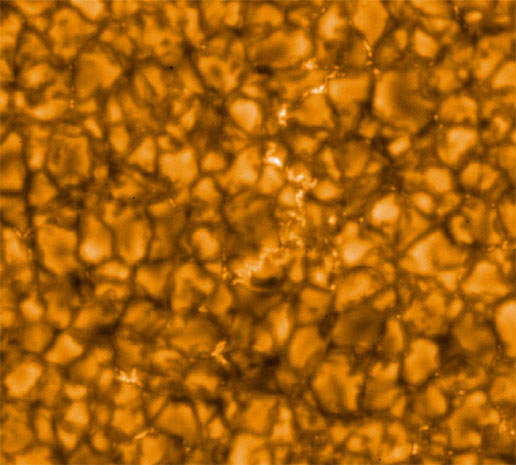
\includegraphics[width=\linewidth]{convection_hinode}
\caption[Solar convection cells]{\label{f.solar-convection} Solar convection cells, imaged with the Hinode Solar Optical Telescope. \imgcred\ Hinode JAXA/NASA/PPARC.}
\end{marginfigure}

\begin{exercisebox}[Temperature and density within a star]
The figure below indicates the central density and temperature (\emph{triangle}) for 3 hypothetical stars: (\emph{left}) a star that is fully convective; (\emph{center}) a star with a radiative (i.e., stable against convection) core (densities greater than $\val{10}{\kilo\gram\usk\meter^{-3}}$) and a convective envelope; (\emph{right}) a star with a convective core and a radiative envelope. For each star, sketch a plausible run of temperature with density within the star. In the center and right panels, the boundary between radiative and convective regions is marked with a vertical solid line.

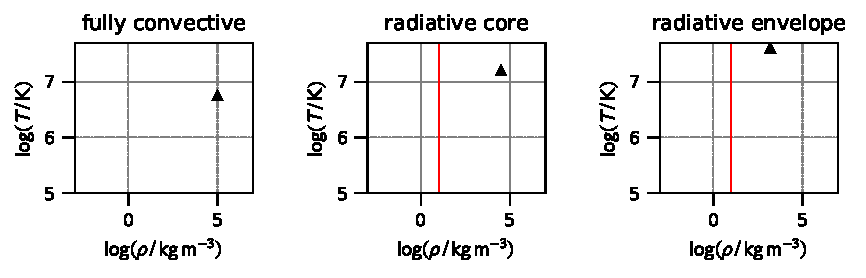
\includegraphics[width=\linewidth]{convection-worksheet-2}
\end{exercisebox}

\newthought{We can now collect the equations describing the structure of a star in steady-state}. Previously, we established the relations for the enclosed mass,
\begin{equation}\label{e.mass}
\DD{m}{r} = 4\pi r^{2}\rho,
\end{equation}
the pressure,
\begin{equation}\label{e.pressure}
\DD{P}{r} = -\rho\frac{Gm}{r^{2}},
\end{equation}
and the luminosity,
\begin{equation}
\label{e.luminosity}
\DD{L}{r} = 4\pi r^{2}\rho\varepsilon.
\end{equation}
To these we add the equations for the temperature,
\begin{eqnarray}\label{e.temperature-radiative}
\DD{T}{r} &=& - \frac{L}{4\pi r^{2}}\frac{3\rho\kappa}{4ac T^{3}}\quad\textrm{where radiative; and}\\
\label{e.temperature-convective}
\DD{T}{r} &\simeq& \frac{T}{P}\tderiv{\ln T}{\ln P}{S}\DD{P}{r}\quad\textrm{where convective}.
\end{eqnarray}
Equations (\ref{e.mass})--(\ref{e.temperature-convective}), or equivalently (\ref{e.lagrange-r})--(\ref{e.lagrange-T-convective}), are supplemented by an equation of state $P = P(\rho,T,\{X\})$, opacity $\kappa = \kappa(\rho,T,\{X\})$, and heating rate $\varepsilon=\varepsilon(\rho,T,\{X\})$. Here $\{X\}$ refers to the mass fractions of the various isotopes. Note that to have a full description we would also need to include equations for the change in composition ($\dif X/\dif t$) due to nuclear burning, as well as terms containing $\dif r/\dif t$ to describe expansion or contraction.

\begin{sidebar}[The equations of stellar structure in Lagrangian form]
\label{sb.lagrangian-equations}
In general, the equations (\ref{e.mass}), (\ref{e.pressure}), (\ref{e.temperature-radiative})-(\ref{e.temperature-convective}), and (\ref{e.luminosity}) must be solved numerically. In practice, the radius $r$ is not the most convenient variable to use as a coordinate. In one dimension, the mass in each shell remains distinct, so the enclosed mass
\[
	m(r) = \int_{0}^{r} 4\pi r^{2}\rho\,\dif r
\]
makes a useful coordinate. Using the enclosed mass as a coordinate is called a \newterm{Lagrangian} description of the star.  Upon changing variables from $r$ to $m$, the structure equations become
\begin{eqnarray}
\DD{r}{m} &=& \frac{1}{4\pi r^{2}\rho}\label{e.lagrange-r}\\
\DD{P}{m} &=& \DD{P}{r}\DD{r}{m} = -\frac{Gm}{4\pi r^{4}}\label{e.lagrange-P}\\
\DD{L}{m} &=& \varepsilon.\label{e.lagrange-L}\\
\DD{T}{m} &=& - \frac{3\kappa L}{64\pi^{2} r^{4} acT^{3}}\qquad \textrm{where radiative}\label{e.lagrange-T-radiative}\\
\DD{T}{m} &\simeq& -\frac{T}{P}\tderiv{\ln T}{\ln P}{S}\frac{Gm}{4\pi r^{4}} \quad \textrm{where convective}\label{e.lagrange-T-convective}
\end{eqnarray}
\end{sidebar}

\section{Contraction to the main sequence}
\label{s.contraction-to-main-sequence}

Stars are formed when clouds of gas and dust fall out of pressure balance and become unstable to gravitational collapse. Often, the cloud fragments into a myriad of small collapsing regions, such as in the Soul and Tauris Nebulae pictured in Fig.~\ref{f.soul-nebula-and-tauris}. In the center of these dense knots, a core comes into hydrostatic equilibrium and grows in mass as matter continues to infall. Much of this process is obscured from view by the surrounding clouds of gas and dust.
\begin{marginfigure}
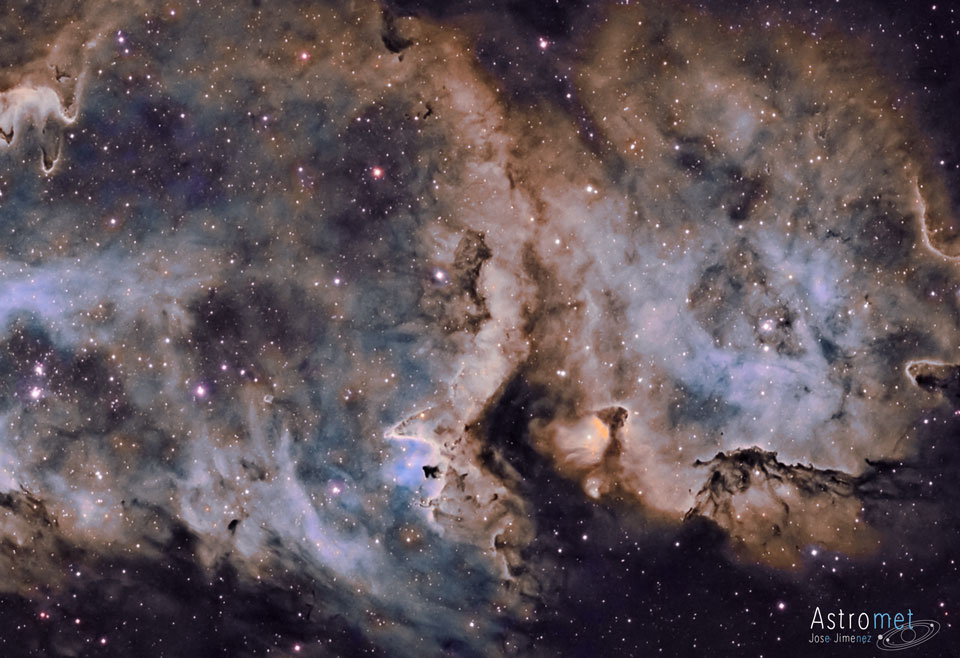
\includegraphics[width=\linewidth]{Soul_Priego_960}
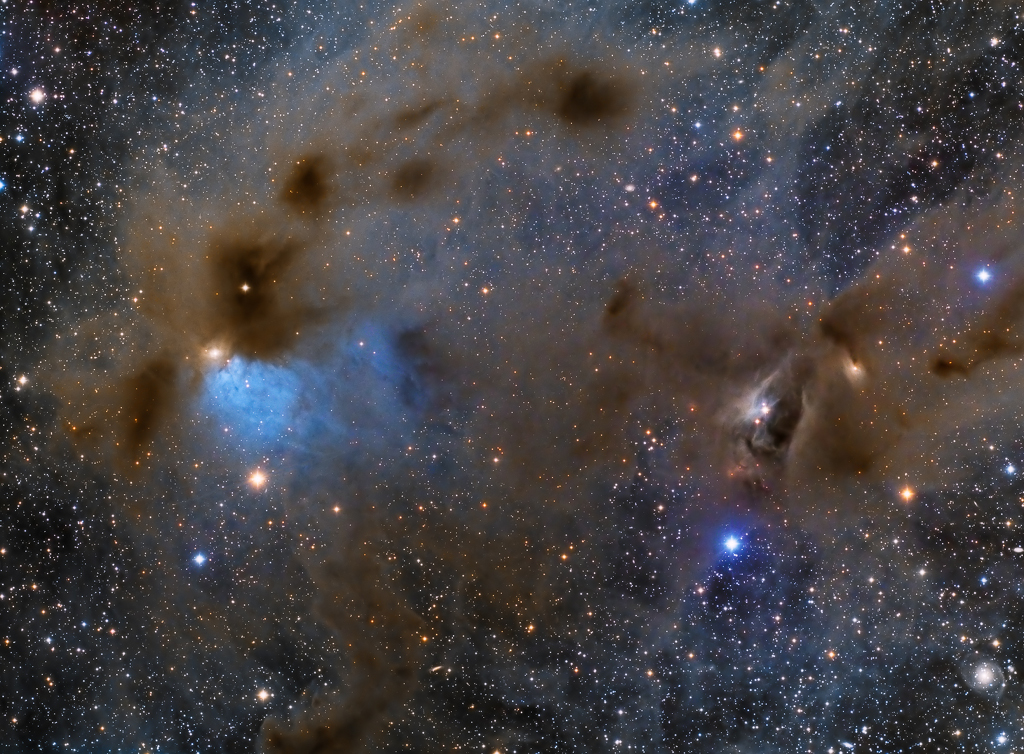
\includegraphics[width=\linewidth]{LBN782ProcessedLRv1-2_1024}
\caption[Pre-main sequence stars]{\label{f.soul-nebula-and-tauris} (Top) Image of the Soul Nebula (IC 1848) in the constellation Cassiopeia. \imgcred\ Jos\'e Jim\'enez Priego (Astromet). (Bottom) The Taurus molecular cloud. At right are million-year old pre-main sequence stars still embedded in dust clouds. \imgcredcopy\ Lloyd L. Smith, Deep Sky West.}
\end{marginfigure}

While the nebula thins out, the pre-main sequence star contracts slowly on a Kelvin-Helmholtz timescale, eq.~(\ref{e.kelvin-helmholtz}), since the core is too cool for nuclear reactions to generate sufficient power. As the central temperature rises, the nuclear reaction rate increases rapidly until the heat released by reactions balances that radiated from the surface. At that point the star joins the \newterm{zero-age main sequence} (ZAMS). Of course, not all collapsing stellar-like objects reach the ZAMS---objects that are too low in mass will not ignite hydrogen fusion, while objects that are too high in mass tend to be unstable and eject mass. We'll now explore these limits in turn.

\begin{exercisebox}[Central temperature and density during contraction]
\label{ex.contraction-to-main-sequence}
This exercise revisits problem~\ref{ex.contraction-constant-density-protostar}. In that exercise you modeled how the density and temperature changed as a pre-main-sequence star contracted. Table~\ref{t.stellar-rhoT} gives central densities and temperatures of stars at the onset of hydrogen fusion (known as the \newterm{zero-age main sequence}). These central temperatures and densities are plotted below and labeled by stellar mass. Assume an ideal-gas equation of state and use the virial relations for the temperature and central density to plot the tracks in this plane each star followed during its contraction.
\begin{center}
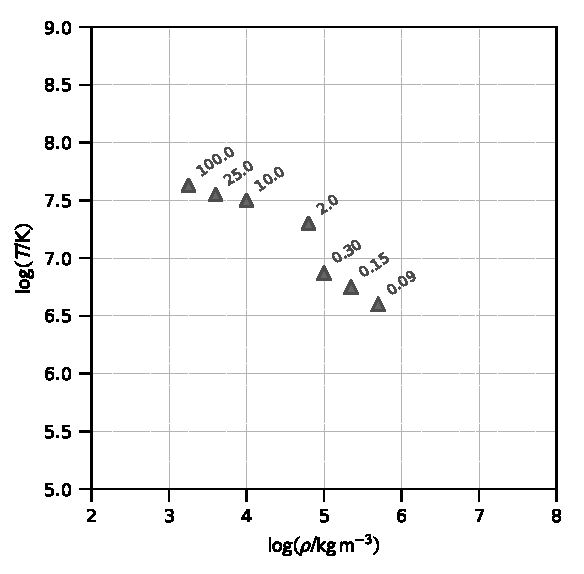
\includegraphics[width=0.8\linewidth]{rho-T-grid}
\end{center}
You will use this plot for exercises \ref{ex.minimum-stellar-mass} and \ref{ex.maximum-stellar-mass} as well.
\end{exercisebox}

\begin{margintable}[-16\baselineskip]
\caption[Central densities and temperatures of zero-age main-sequence stars]{\label{t.stellar-rhoT}Selected central densities and temperatures of zero-age main-sequence stars, computed with the \mesa\ stellar evolution code \citep{Paxton2010Modules-for-Exp}.}
\begin{tabular}{rrr}
$M/\Msun$ & $\log(\rho_{c}/\kilo\gram\,\meter^{-3})$ & $\log(T_{c}/K)$\\
\hline
0.09 & 5.70 & 6.60\\
0.15 & 5.35 & 6.75\\
0.30 & 5.00 & 6.87\\
2.0 & 4.80 & 7.30\\
10.0 & 4.00 & 7.50\\
25.0 & 3.60 & 7.55\\
100.0 & 3.25 & 7.63\\
\end{tabular}
\end{margintable}

\subsection{Degeneracy}
\label{s.degeneracy}

As a star contracts, the particles within it are packed ever closer together.  As we saw from our discussion of ionization, quantum mechanics enters the description of particle behavior when the separation between particles is of the order of the uncertainty in their positions.  Said differently, our classical description breaks down when the particle density exceeds roughly
\begin{equation}\label{e.heuristic-quantum-density}
    n > \frac{1\;\textrm{particle}}{(\Delta x)^3} 
    = \left(\frac{\Delta p}{h}\right)^3 
    \approx \left(\frac{m\kB T}{h^2}\right)^{3/2}.
\end{equation}
Another way to put this is that quantum effects become important when there is more than roughly 1 particle in a normalized phase space volume $\dif^{3}x\,\dif^{3}p/h^{3}$.

If the particles are this densely packed, their wavefunctions overlap and we must describe the system as a single quantum state.
Suppose we have two identical particles in a quantum state. Since the particles are identical, if we exchange them the wavefunction can only change by a phase factor\sidenote{See Box~\ref{sb.identical-particles}} $e^{i\delta}$. If we exchange the particles again, we are back to our original state; as a result, $e^{2i\delta} = 1$, and therefore $\delta = 0$ or $\pi$. Hence upon the exchange of particles, the wavefunction either is unchanged ($\delta=0,e^{i\delta}=1$) or it changes sign ($\delta=\pi,e^{i\pi}=-1$).
\begin{quote}\itshape
    There are two types of wavefunctions in this world: those that change sign under exchange; and those that don't.
\end{quote}
Particles whose wavefunctions don't change sign under exchange are called \newterm{bosons} and have integer spin. Photons ($\textrm{spin} = 1$) are bosons. Particles whose wavefunctions change sign under exchange are called \newterm{fermions} and have half-integer spin. Electrons, neutrinos, protons, and neutrons ($\textrm{spin} = 1/2$) are all fermions. 

A consequence of the fermion wavefunction changing sign when any two particles are exchanged is that the wavefunction vanishes if any two particles are in the same state---that is, they have the same position, momentum, and spin. For spin-half particles like electrons, this means we can put at most two such electrons in the same position and momentum state; we do this by having their spins antiparallel.

\begin{sidebar}[Identical particles]
\label{sb.identical-particles}
To understand how the interchange of identical particles works in more detail, let's start by recalling some features of quantum mechanics. This discussion is based on  \citet{Feynman1989The-Feynman-Lec}.
We denote a particle's state as $\ket{a}$, where $a$ is just a label.  For example, $a$ could be "electron with such-and-such properties".  The probability of finding the electron in some other state $\ket{\phi}$ is given by $|\braket{\phi}{a}|^2$, where $\braket{\phi}{a}$ is a complex number known as the probability amplitude formed via an inner product of $\ket{\phi}$ and $\ket{a}$.

Now suppose we have two particles, a and b, and we scatter them so that one particle ends up in detector 1 and the other ends up in detector 2. There are two ways this can go, as shown here.
\begin{center}
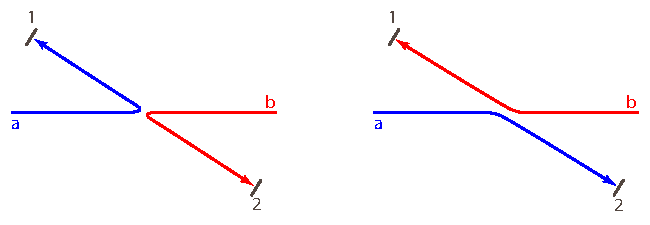
\includegraphics[width=\linewidth]{scattering-classical}
\end{center}
Classically, we would argue that the probability of getting either particle in detector 1 is just
\begin{equation}
    \mathcal{P}(\textrm{a or b in 1}) = \mathcal{P}(\textrm{a in 1}) + \mathcal{P}(\textrm{b in 1}).
\end{equation}
If particles a and b are different---e.g., one is a \carbon\ nucleus and the other is an \oxygen\ nucleus---then this holds in quantum mechanics as well. Quantum mechanically, we write
\begin{equation}\label{e.classical-probability}
    \mathcal{P}(\textrm{a or b in 1}) = |\braket{1}{a}\braket{2}{b}|^2 + |\braket{2}{a}\braket{1}{b}|^2.
\end{equation}
If the particles are identical, however---for example, if a and b are two electrons with identical spin---then this picture is wrong.

Because of the uncertainty principle, we cannot follow the trajectories of a and b with infinite precision to see which is which; instead, the situation is more analogous to the depiction shown here.
\begin{center}
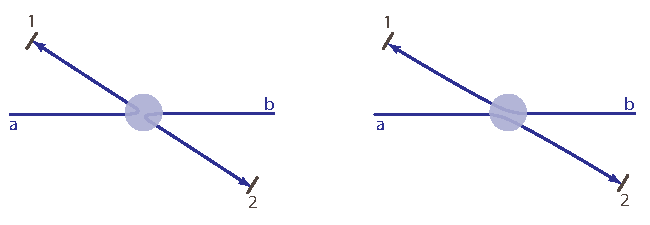
\includegraphics[width=\linewidth]{scattering-quantum}
\end{center}
There are now two indistinguishable ways of arriving at the final state---in this case, an electron in detector 1 and an electron in detector 2. According to quantum mechanics, we must therefore sum the amplitudes for getting to the final state, \emph{before taking the square}. That is, the probability for this one particle to end up in detector 1 and the other to end up in detector 2 is
\begin{eqnarray}
    \lefteqn{\mathcal{P}(\textrm{a or b in 1}) = |\braket{1}{a}\braket{2}{b} + \braket{2}{a}\braket{1}{b}|^2} && \label{e.scattering-quantum}\\
    &=& |\braket{1}{a}\braket{2}{b}|^2 + |\braket{2}{a}\braket{1}{b}|^2 \nonumber\\
    && + {\color{red}\left[ \braket{1}{a}^*\braket{2}{b}^*\braket{2}{a}\braket{1}{b} + \braket{2}{a}^*\braket{1}{b}^*\braket{1}{a}\braket{2}{b}\right]}. \nonumber
\end{eqnarray}
The probability of scattering one electron into detector 1 and the other into detector 2 is the  value for distinguishable particles, eq.~(\ref{e.classical-probability}), \emph{plus} an interference term in $\color{red}[\cdot]$.

\newthought{To see the effect of this interference term on the thermal properties of the system,} let's imagine putting two particles into the same small volume.  To do this, we imagine the detectors 1 and 2 sliding together until they overlap, as shown here.  
\begin{center}
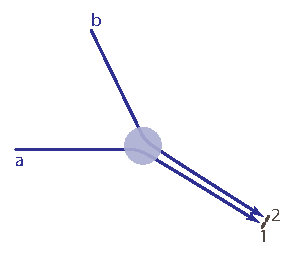
\includegraphics{fermions}
\end{center}
Since detectors 1 and 2 are approaching one another, we must have
\begin{equation}
    |\braket{1}{a}\braket{2}{b}|^2 = |\braket{2}{a}\braket{1}{b}|^2.
\end{equation}
This does not imply, however, that $\braket{1}{a}\braket{2}{b} = \braket{2}{a}\braket{1}{b}$: the amplitudes could differ by a phase factor, so that interchanging the particles would yield
\[
    \braket{2}{a}\braket{1}{b} = e^{i\delta}\braket{1}{a}\braket{2}{b}.
\]
If we interchange the particles, and then interchange them again, we get
\[
    \braket{1}{a}\braket{2}{b} = e^{2i\delta}\braket{1}{a}\braket{2}{b};
\]
since swapping the particles twice just gets up back to the original situation, we must have that $e^{2i\delta} = 1$ and therefore $e^{i\delta} = \pm 1$.

If there is no change of sign, i.e., $\braket{2}{a}\braket{1}{b} = \braket{1}{a}\braket{2}{b}$, then from equation~(\ref{e.scattering-quantum}) we have
\begin{equation}\label{e.boson}
    \mathcal{P}(\textrm{a or b in 1}) = 2\left(|\braket{1}{a}\braket{2}{b}|^2 + |\braket{2}{a}\braket{1}{b}|^2\right).
\end{equation}
This is \emph{twice} the classical value: the probability of the particles entering the same state is enhanced.

In contrast, if the sign changes under exchange, i.e., if $\braket{2}{a}\braket{1}{b} = -\braket{1}{a}\braket{2}{b}$, then equation~(\ref{e.scattering-quantum}) implies that
\begin{eqnarray}
\mathcal{P}(\textrm{a or b in 1}) &=& |\braket{1}{a}\braket{2}{b}|^{2} + |\braket{2}{a}\braket{1}{b}|^{2} \nonumber\\ 
    && - |\braket{1}{a}\braket{2}{b}|^{2} - |\braket{2}{a}\braket{1}{b}|^{2} \nonumber\\ 
    &=& 0.\label{e.fermion}
\end{eqnarray}
\begin{quote}\itshape
We cannot have 2 identical particles with the same momentum, position, and spin if their wavefunction changes sign when the particles are exchanged.
\end{quote}
Particles with integer spin (i.e., their angular momentum is an integer multiple of $\hbar$) have wavefunctions that do not change sign under exchange; these particles are said to obey \newterm{Bose-Einstein statistics} and are called \newterm{bosons}.  Particles with half-integer spin have wavefunctions that do change sign under exchange; these particles are said to obey \newterm{Fermi-Dirac statistics} and are called \newterm{fermions}.  Photons are bosons; electrons, protons, neutrons, and neutrinos are fermions.
\end{sidebar}

\newthought{To account for Fermi-Dirac statistics within the equation of state,} we imagine a small volume containing $N$ electrons. Motivated by eq.~(\ref{e.heuristic-quantum-density}), we divide the phase space into cells,
\[
	\frac{\dif^{3}x\,\dif^{3}p}{h^{3}},
\]
and into each cell we place 2 electrons with opposing spins. We always add the electrons to the lowest open energy level, and repeat the process until we have added all $N$ electrons. This procedure is represented by the equation
\begin{equation}
\label{e.number-degenerate}
	N = \frac{2}{h^{3}}\int_{V}\dif^{3}x\int_{0}^{\EF}\dif^{3}p
\end{equation}
In this equation $\EF$, the \emph{Fermi energy}, is the energy of the last electron added and is the largest filled energy level.

If our volume is isotropic, then we can change variables: first, to spherical momentum coordinates, $\dif^{3}p = 4\pi p^{2}\,\dif p$; second, from $\dif p$ to $\dif\varepsilon$.  Since $p = \sqrt{2m\varepsilon}$, where $\varepsilon$ is the energy of a single electron,
\[
	\dif p = \sqrt{\frac{m}{2\varepsilon}}\,\dif \varepsilon;
\]
upon changing variables and integrating over $\varepsilon$ from $0$ to $\EF$ we obtain
\[
	N = \frac{8\pi}{h^{3}}V \int_{0}^{\EF} \sqrt{2}m^{3/2}\varepsilon^{1/2}\,\dif \varepsilon
	= \frac{8\pi}{3h^{3}} V (2m)^{3/2} \EF^{3/2}.
\]
Solving for the Fermi energy gives
\begin{equation}\label{e.fermi-energy}
	\EF = \frac{h^{2}}{2m}\left(\frac{3}{8\pi}\frac{N}{V}\right)^{2/3}.
\end{equation}
What is the total energy of our system? We again integrate over phase space, with each electron multiplied by its energy $\varepsilon$:
\begin{equation}\label{e.total-energy}
	E = \frac{8\pi}{h^{3}}V\int_{0}^{\EF}\sqrt{2}m^{3/2}\varepsilon^{3/2}\,\dif\varepsilon = \frac{8\pi}{5h^{3}}V(2m)^{3/2} \EF^{5/2}.
\end{equation}
Using eq.~(\ref{e.fermi-energy}) to substitute for $\EF$ in eq.~(\ref{e.total-energy}), we can find the energy per unit volume,
\[
	\frac{E}{V} = \frac{3}{5}\left(\frac{3}{8\pi}\right)^{2/3}\frac{h^{2}}{2m}n^{5/3} = \frac{3}{5} n \EF,
\]
where $n=N/V$ is the density of electrons.

For a non-relativistic gas the pressure is $P = (2/3)(E/V)$.  Hence the pressure of our electron gas is
\begin{equation}\label{e.pressure-electrons}
	P = \frac{2}{3}\frac{E}{V} = \frac{2}{5} n\EF
		= \frac{2}{5}\left(\frac{3}{8\pi}\right)^{2/3}\frac{h^{2}}{2m}n^{5/3}.
\end{equation}
Notice that the pressure is independent of the temperature.

Electrons, being more than 1000 times lighter than nuclei, become degenerate first. Suppose our composition consists of species with charge $Z_{i}$ and mass number $A_{i}$. Then the number of electrons per unit volume\sidenote{assuming complete ionization} is
\[
	n_{e} = \sum_{i} n_{i} Z_{i} = \frac{\rho}{\mb}\sum_{i} X_{i}\frac{Z_{i}}{A_{i}}.
\]
By analogy with the mean molecular weight, we define an electron mean weight
\begin{equation}\label{e.electron-mean-weight}
\mu_{e} \equiv \left(\sum_{i}X_{i}\frac{Z_{i}}{A_{i}}\right)^{-1}
\end{equation}
so that $n_{e} = \rho/(\mb\mu_{e})$. Equation~(\ref{e.pressure-electrons}) then provides a relationship between pressure and density for a given $\mu_{e}$.

\begin{exercisebox}[The mass-radius relation for a degenerate EOS]
\label{ex.degenerate-mass-radius}
Express the pressure as a function of mass density $\rho$ and $\mu_{e}$. Then use the virial scalings for $P(M,R)$ and $\rho(M,R)$ to obtain a relation $R(M)$ for a degenerate object.
\end{exercisebox}

As you found in exercise~\ref{ex.degenerate-mass-radius}, when the star becomes degenerate, there is a unique radius for a given mass and composition. This is in contrast to the non-degenerate case, for which a star of a given mass can have a wide range of possible radii depending on the internal temperature.

Consider a contracting pre-main-sequence star. Initially, the star has a low density and the equation of state is that of an ideal non-degenerate gas. According to the virial theorem, as the radius decreases, both the central temperature and density increase. 
The radius decreases because the star is radiating away energy, and a star with an ideal, non-degenerate equation of state has a total energy that depends on its radius.

At some density, the equation of state will become degenerate. At this point, contraction comes to a halt. The star continues to radiate energy, but instead of contracting, the star simply cools while remaining at constant radius. If the contracting pre-main-sequence star is to become a main-sequence star, then, it must reach temperatures sufficient for hydrogen fusion to occur \emph{before} becoming degenerate.

\begin{exercisebox}[Minimum stellar mass]
\label{ex.minimum-stellar-mass}
The equation of state becomes degenerate roughly where $\kB T=\EF$, with $\EF$ begin given by eq.~(\ref{e.fermi-energy}). From this and eq.~(\ref{e.electron-mean-weight}), assuming a H-He composition with $X_{\mathrm{H}} = 0.7$ and $X_{\mathrm{He}}=0.3$, derive a relation between $\log(T)$ and $\log(\rho)$. Plot this relation on the phase diagram in exercise~\ref{ex.contraction-to-main-sequence}, and on the plot indicate which side of the relation is degenerate.
Given that contraction halts when the equation of state becomes degenerate, what does this plot imply for the minimum mass required to initiate hydrogen fusion?
\end{exercisebox}

\newthought{As shown in exercise \ref{ex.minimum-stellar-mass}, there is a minimum mass needed to initiate hydrogen fusion.} Contracting star-like objects of lower mass are known as \newterm{brown dwarfs}. Although dim, they are observable with spectral types ``L'', ``T'' or ``Y''\cite{Kirkpatrick1999Dwarfs-Cooler-t,Cushing2011The-Discovery-o}.

\begin{exercisebox}[Planetary masses and radii]
\label{ex.planetary-M-and-R}
You might notice that the degenerate mass-radius relation you found in exercise~\ref{ex.degenerate-mass-radius} can't hold for very light objects (or very heavy ones, for that matter). Earth, for example has a much larger mass than Mars, and also has a larger radius, contrary to what the degenerate relation predicts. What happens is that at low pressures, the Coulomb force comes into play---the atomic and molecular bonds that add variety to life. These bonds set the size and spacing of atoms, and therefore fix the density of matter. Let's model this. The typical size of an atom is the Bohr radius,
\[
	a_{\mathrm{B}} = \frac{4\pi\varepsilon_{0}\hbar^{2}}{m_{e}e^{2}} = \val{\sci{5.29}{-11}}{\meter}.
\]
	\begin{enumerate}
	\item Let take our mass density as being one average nuclear mass per volume $a_{\mathrm{B}}^{3}$.  We'll again use our solar composition, $X_{\mathrm{H}}=0.7, X_{\mathrm{He}}=0.3$.
What is the value of this density? Is it plausible?
	\item If matter is at this density, what is $R(M)$?
	\item Roughly for what mass object, if any, does this $R(M)$ relation intersect the relation for degenerate matter? This sets the mass at which degeneracy becomes important for a cold object. Compare this mass with objects in the solar system.
	\end{enumerate}
\end{exercisebox}

\subsection{Radiation pressure}
\label{s.radiation-pressure}

\begin{marginfigure}
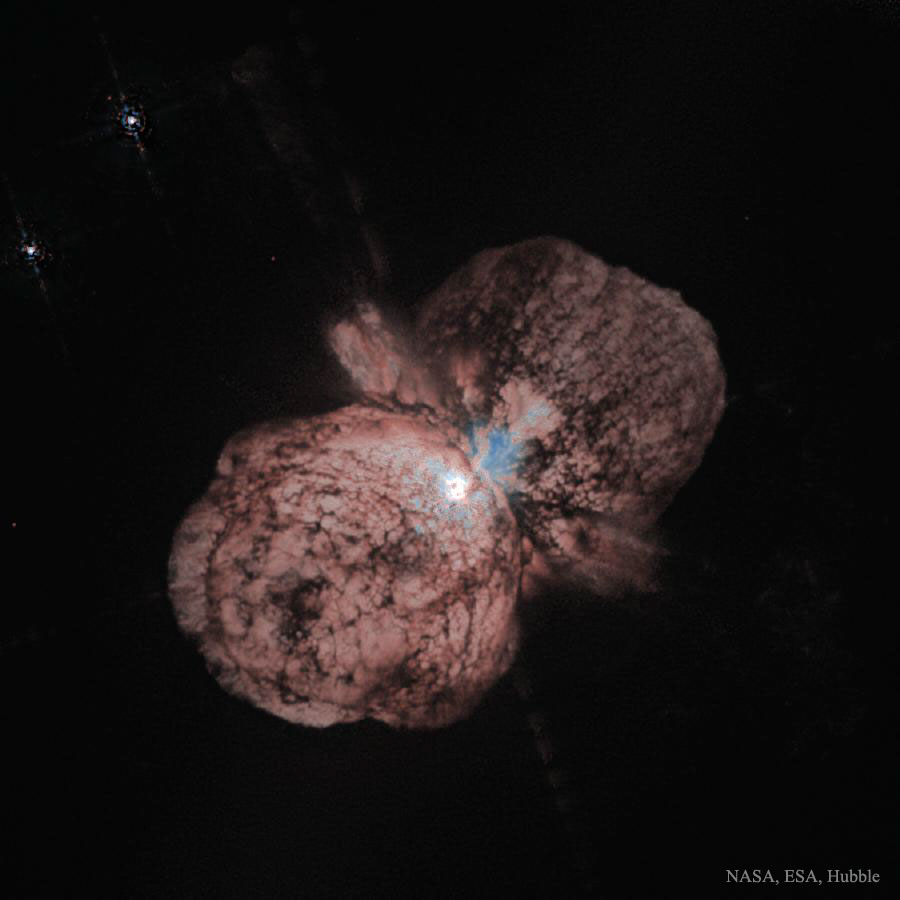
\includegraphics[width=\linewidth]{etacarinae_hubble_900}
\caption[Image of the massive star Eta Carinae]{\label{f.eta-carinae} Image of the massive star Eta Carinae. \imgcred\ J. Morse (Arizona State U.), K. Davidson (U. Minnesota) et al., WFPC2, HST, NASA.}
\end{marginfigure}
Radiation in thermal equilibrium exerts a pressure (eq.~\ref{e.radiation-pressure}): $\Prad = aT^{4}/3$. Because of this strong dependence on temperature, radiation pressure becomes an increasingly large fraction of the total pressure for massive stars. Stars that are radiation-pressure dominated tend to be unstable: they have strong winds and violent fits of mass ejection (see the image of Eta Carinae, Fig.~\ref{f.eta-carinae}). As a result, they lose copious amounts of mass while on the main sequence. This mass-shedding effectively sets a rough upper limit to the range of main-sequence stellar masses.

\begin{exercisebox}[Radiation pressure]
Use the virial relations for density and temperature to estimate how the ratio $\Prad/P_{\!\mathrm{gas}}$ depends on the mass of the star.
\end{exercisebox}

\begin{exercisebox}[Maximum stellar mass]
\label{ex.maximum-stellar-mass}
The equation of state becomes dominated by radiation roughly where $P(\textrm{ideal gas}) \approx P(\textrm{radiation})$. Derive from this criterion a relation between $\log(T)$ and $\log(\rho)$, and plot this relation on the figure for exercise~\ref{ex.contraction-to-main-sequence}. Indicate which side of this relation is radiation-pressure dominated. What do your findings in this exercise imply for the mass range of main-sequence stars?
\end{exercisebox}

\section{Life on the main-sequence}

With the initiation of hydrogen fusion, the star settles into thermal and mechanical equilibrium, with its structure described by the solution of equations\sidenote{Or, in Lagrangian form, (\ref{e.lagrange-r})--(\ref{e.lagrange-L}).} (\ref{e.mass})--(\ref{e.luminosity}), along with the equation of state and prescriptions for the opacity $\kappa$ and heating rate $\varepsilon$. 

The reason for star's stability on the main sequence is a consequence of the relation, derived in exercise \ref{ex.gravithermal-specific-heat}, between the star's total energy and temperature. If the reaction rate were to increase and deposit more energy into the star, then since the total energy is $\propto -GM^{2}/R$, the star would expand. This expansion would cause the central temperature to decrease, thereby reducing the reaction rate.

The star is not in complete equilibrium, however, as hydrogen in the core is gradually being converted to helium. The timescale over which the composition changes is much longer than the dynamical timescale (sets hydrostatic equilibrium), the radiative diffusion timescale (sets thermal gradient), and the Kelvin-Helmholtz timescale (sets core temperature via growth or contraction of stellar radii). The gradual build-up of a helium-rich core does not, therefore, affect the stability of the star, but it does lead to a slow brightening of the star over its main sequence lifetime. For our sun, the gradual enrichment of the core in helium causes a slow increase in luminosity of $\approx10\%$ for each billion years.\marginnote{Although this slow increase in luminosity is not a drastic change, it has significant implications for life on Earth. The expected warming is sufficient to make Earth uninhabitable within about a billion years from now.} 

\begin{exercisebox}[Nuclear burning timescale]
\label{ex.nuclear-burning-timescale}
You computed in exercise \ref{ex.Q-hydrogen-helium} the energy released from the conversion of 4 hydrogen atoms into helium. Express this number in terms of the energy released per mass of hydrogen burned; this number should be in units of $\unitstyle{J}/\kilo\gram$. Now assume that the sun's luminosity comes from the fusion of hydrogen into helium in the innermost 10\% of the sun's mass. For a composition that is 70\% hydrogen by mass, how long would it take to deplete the hydrogen in the solar core? This sets the main-sequence lifetime of the sun.
\end{exercisebox}

The cool outer layers of low-mass stars have large opacities: for example many elements are not ionized, so there are many potential lines for absorption. As a result, stars with $M\lesssim\Msun$ have convective regions in their outer parts. The fraction of the star that is convective is larger for low-mass, cool stars; and stars with $M \lesssim\val{0.3}{\Msun}$ are fully convective, so that the whole interior lies along an adiabat. For more massive, hotter, stars, the opacities are lower, and as a result, the outer convective region vanishes for stars with $M\gtrsim\Msun$.

\begin{exercisebox}[Mass-luminosity relation]
\label{ex.mass-luminosity-relation}
We can estimate how the luminosity depends on stellar mass for stars that have a mostly radiative structure. Start with equation (\ref{e.temperature-radiative}) for the temperature gradient and approximate $\dif T/\dif r \approx T_{c}/R$, $\rho \approx \bar{\rho}$, $L/4\pi r^{2} \approx L/4\pi R^{2}$, and $T\approx T_{c}$. Take the opacity $\kappa$ to be constant,  use the virial estimate for the central temperature $T_{c}$ and express the mean density $\bar{\rho}$ in terms of stellar mass $M$ and radius $R$. After some algebra, you should find that the luminosity $L$ depends on $M$ to some power. Compare this scaling against the data in Table~\ref{t.stellar-properties}. Obtain an expression for the stellar lifetime as a function of mass, and calibrate it to the sun's main-sequence lifetime, $\tau_{\odot}\sim\val{10}{\Giga\yr}$.
\end{exercisebox}

\newthought{Stars more massive than the sun have sufficiently high core temperatures for hydrogen to be consumed via the CNO cycle.} The strong temperature dependence of the CNO burning has two effects on the structure of the star. First, it makes the central temperature nearly constant over a wide range of stellar masses for $M>\val{1}{\Msun}$---a small rise in temperature is sufficient to raise the heat production $\varepsilon$ to match the rise in luminosity. A nearly constant central temperature implies, via the virial theorem, that $R \propto M$ on the upper main sequence. The second consequence is that nearly all of the star's luminosity is generated in a small region about the stellar center. The flux, $L/4\pi r^{2}$, in this small region is enormous, and this makes the core of the star convective. The convection can mix hydrogen fuel into the core, which makes the lifetime somewhat longer than the estimate from exercise~\ref{ex.mass-luminosity-relation}. A summary of the structure of main sequence stars is contained in Table~\ref{t.MS-characteristics}.
\begin{margintable}
\caption{\label{t.MS-characteristics} Characteristics of main-sequence stars}
\centering
\begin{tabular}{lll}
 & $M\lesssim\Msun$ & $M\gtrsim\Msun$\\
\hline
$4\pt\to\helium$\ldots & pp & CNO\\
core is\ldots & radiative  & convective\\
envelope is\ldots & convective & radiative\\
\end{tabular}
\end{margintable}


